% vim: set spell spelllang=en tw=100 et sw=4 sts=4 :

\documentclass[a0paper]{tikzposter}

\usepackage{algorithm2e,algpseudocode}
\usepackage{complexity}
\usepackage{wrapfig}
\usepackage{microtype}
\usepackage{gnuplot-lua-tikz}
\usepackage{amssymb}
\usepackage{amsmath}
\usepackage{sfmath}

\usepackage{lmodern}
\renewcommand*\familydefault{\sfdefault}
\usepackage[T1]{fontenc}

\newcommand{\McSplit}{\textproc{McSplit}}

\title{A Partitioning Algorithm for Maximum Common Subgraph Problems}
\author{Ciaran McCreesh, Patrick Prosser and James Trimble}
\institute{University of Glasgow, Glasgow, Scotland}
\titlegraphic{
\includegraphics[keepaspectratio=true,scale=3.5]{UoG_keyline.pdf}}

\settitle{
    \begin{tikzpicture}
        \node (T) [inner sep=0pt] {\begin{minipage}{\linewidth}
                \color{titlefgcolor}
                {\bfseries \Huge \hspace*{10mm}A Partitioning Algorithm for Maximum \\
                \hspace*{10mm}Common Subgraph Problems \par}
                \vspace*{1em}
                {\Large {\bfseries \hspace{10mm}\@author}, \@institute}
        \end{minipage}};

        \node at (T.east) [anchor=center, inner sep=0pt, xshift=-12cm] {\@titlegraphic};
    \end{tikzpicture}
}

% University of Glasgow standard colours
\definecolor{uofguniversityblue}{rgb}{0, 0.219608, 0.396078}

\definecolor{uofgheather}{rgb}{0.356863, 0.32549, 0.490196}
\definecolor{uofgaquamarine}{rgb}{0.603922, 0.72549, 0.678431}
\definecolor{uofgslate}{rgb}{0.309804, 0.34902, 0.380392}
\definecolor{uofgrose}{rgb}{0.823529, 0.470588, 0.709804}
\definecolor{uofgmocha}{rgb}{0.709804, 0.564706, 0.47451}

\definecolor{uofglawn}{rgb}{0.517647, 0.741176, 0}
\definecolor{uofgcobalt}{rgb}{0, 0.615686, 0.92549}
\definecolor{uofgturquoise}{rgb}{0, 0.709804, 0.819608}
\definecolor{uofgsunshine}{rgb}{1.0, 0.862745, 0.211765}
\definecolor{uofgpumpkin}{rgb}{1.0, 0.72549, 0.282353}
\definecolor{uofgthistle}{rgb}{0.584314, 0.070588, 0.447059}
\definecolor{uofgpillarbox}{rgb}{0.701961, 0.047059, 0}
\definecolor{uofglavendar}{rgb}{0.356863, 0.301961, 0.580392}

\definecolor{uofgsandstone}{rgb}{0.321569, 0.278431, 0.231373}
\definecolor{uofgforest}{rgb}{0, 0.317647, 0.2}
\definecolor{uofgburgundy}{rgb}{0.490196, 0.133333, 0.223529}
\definecolor{uofgrust}{rgb}{0.603922, 0.227451, 0.023529}

\definecolorstyle{UofG}{
}{
    % Background Colors
    \colorlet{backgroundcolor}{uofgsandstone!80!white}
    \colorlet{framecolor}{black}
    % Title Colors
    \colorlet{titlefgcolor}{white}
    \colorlet{titlebgcolor}{uofguniversityblue}
    % Block Colors
    \colorlet{blocktitlebgcolor}{white}
    \colorlet{blocktitlefgcolor}{uofguniversityblue}
    \colorlet{blockbodybgcolor}{white}
    \colorlet{blockbodyfgcolor}{black}
    % Innerblock Colors
    \colorlet{innerblocktitlebgcolor}{uofguniversityblue}
    \colorlet{innerblocktitlefgcolor}{black}
    \colorlet{innerblockbodybgcolor}{uofgsandstone}
    \colorlet{innerblockbodyfgcolor}{black}
    % Note colors
    \colorlet{notefgcolor}{black}
    \colorlet{notebgcolor}{uofgrust}
    \colorlet{noteframecolor}{red}
}

\usetheme{Autumn}
\usecolorstyle{UofG}

\tikzposterlatexaffectionproofoff

\useblockstyle[bodyverticalshift=-1cm, roundedcorners=1]{Default}

\renewcommand{\Huge}{\fontsize{77.2}{96}\selectfont}

% Styles for drawings

\tikzset{edge/.style={line width=3pt, color=uofgsandstone}}
\tikzset{ledge/.style={line width=3pt, color=uofgsandstone!40!white}}
\tikzset{hedge/.style={line width=3pt, color=uofgsandstone, dashed}}

\setlength\intextsep{0pt}

\begin{document}
\maketitle

{
    \colorlet{blockbodybgcolor}{uofgcobalt}
    \colorlet{blocktitlebgcolor}{uofgcobalt}
    \block[bodyverticalshift=0cm, bodyinnersep=3mm]{}{
        \centering\begin{minipage}{0.94\textwidth}
            We introduce a new branch and bound algorithm for the \textbf{maximum common
            subgraph} and \textbf{maximum common connected subgraph} problems which is based
            around vertex labelling and partitioning. Our method resembles
            a constraint programming approach, but uses a novel compact
            domain store to reduce
            the memory and computation requirements during search.  Experiments
            show a speedup of more than an order of magnitude over the state of the
            art, and demonstrate that we can operate on much larger graphs without
            running out of memory.
%            We show how to generate \textbf{really hard} random instances for \textbf{subgraph
%            isomorphism} problems. For the non-induced variant, we predict and observe a phase
%            transition between satisfiable and unsatisfiable instances, with a corresponding
%            complexity peak seen in \textbf{three different solvers}. For the induced variant, much
%            richer behaviour is observed, and \textbf{constrainedness} gives a better measure of
%            difficulty than does proximity to a phase transition. We also discuss \textbf{variable
%            and value ordering} heuristics, and their relationship to the \textbf{expected number of
%            solutions}.
        \end{minipage}
    }
}

\begin{columns}
\column{0.5}

\block{The Maximum Common Subgraph Problem}{
\begin{wrapfigure}[7]{r}{0.46\linewidth}
    \begin{center}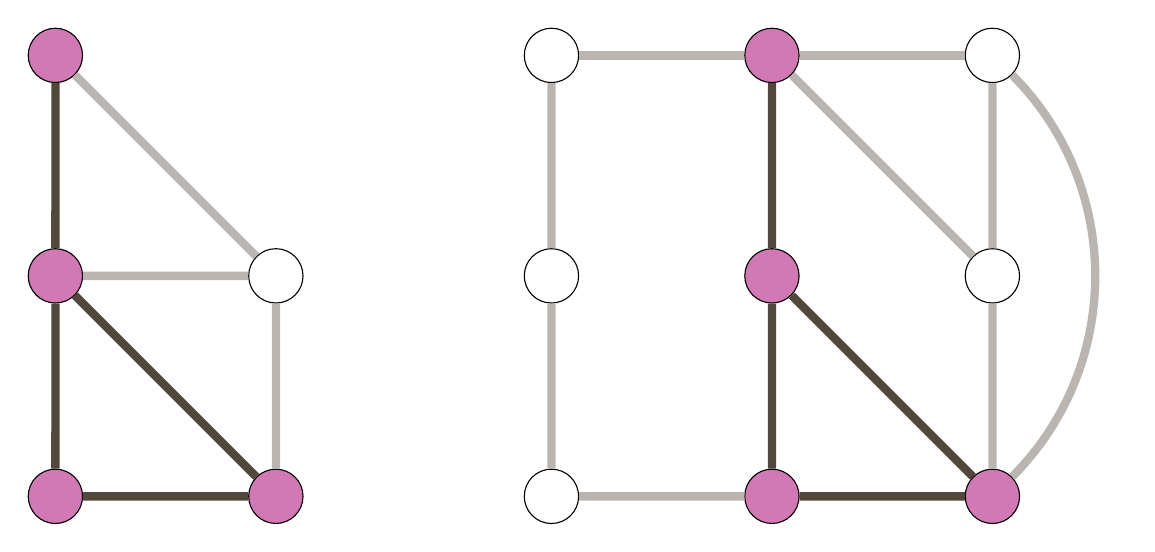
\begin{tikzpicture}[scale=1.4]%{{{
        \node[draw, circle, fill=uofgrose, inner sep=5pt, font=\bfseries] (Na) at (1,  0)
        {\vphantom{0}};
        \node[draw, circle, fill=uofgrose, inner sep=5pt, font=\bfseries] (Nb) at (1, -2)
        {\vphantom{0}};
        \node[draw, circle, fill=uofgrose, inner sep=5pt, font=\bfseries] (Nc) at (1, -4)
        {\vphantom{0}};
        \node[draw, circle, fill=uofgrose, inner sep=5pt, font=\bfseries] (Nd) at (3, -4)
        {\vphantom{0}};
        \node[draw, circle, fill=white, inner sep=5pt, font=\bfseries] (Ne) at (3, -2)
        {\vphantom{0}};

        \draw [edge] (Na) -- (Nb);
        \draw [edge] (Nb) -- (Nc);
        \draw [edge] (Nc) -- (Nd);
        \draw [edge] (Nb) -- (Nd);
        \draw [ledge] (Na) -- (Ne);
        \draw [ledge] (Nb) -- (Ne);
        \draw [ledge] (Nd) -- (Ne);

        \node[draw, circle, fill=uofgrose, inner sep=5pt, font=\bfseries] (N1) at (7.5,  0) {\vphantom{0}};
        \node[draw, circle, fill=white, inner sep=5pt, font=\bfseries] (N2) at (9.5,  0) {\vphantom{0}};
        \node[draw, circle, fill=uofgrose, inner sep=5pt, font=\bfseries] (N3) at (7.5, -2) {\vphantom{0}};
        \node[draw, circle, fill=white, inner sep=5pt, font=\bfseries] (N4) at (9.5, -2) {\vphantom{0}};
        \node[draw, circle, fill=uofgrose, inner sep=5pt, font=\bfseries] (N5) at (7.5, -4) {\vphantom{0}};
        \node[draw, circle, fill=uofgrose, inner sep=5pt, font=\bfseries] (N6) at (9.5, -4) {\vphantom{0}};
        \node[draw, circle, fill=white, inner sep=5pt, font=\bfseries] (N7) at (5.5,  0) {\vphantom{0}};
        \node[draw, circle, fill=white, inner sep=5pt, font=\bfseries] (N8) at (5.5, -2) {\vphantom{0}};
        \node[draw, circle, fill=white, inner sep=5pt, font=\bfseries] (N9) at (5.5, -4) {\vphantom{0}};

        \draw [ledge] (N1) -- (N2);
        \draw [edge] (N1) -- (N3);
        \draw [ledge] (N1) -- (N4);
        \draw [ledge] (N2) -- (N4);
        \draw [edge] (N3) -- (N5);
        \draw [edge] (N3) -- (N6);
        \draw [ledge] (N4) -- (N6);
        \draw [edge] (N5) -- (N6);
        \draw [ledge] (N2) to [in=45, out=315] (N6);
        \draw [ledge] (N1) -- (N7);
        \draw [ledge] (N5) -- (N9);
        \draw [ledge] (N7) -- (N8);
        \draw [ledge] (N8) -- (N9);
    \end{tikzpicture}\end{center}

\end{wrapfigure}

The \textbf{maximum common subgraph} family of problems involves finding a large
graph which is isomorphic to subgraphs of two given graphs simultaneously.
Because graphs are widely used to model real-world phenomena, maximum common
subgraph problems have arisen in molecular science (where graphs often represent
molecules)
and also in other domains including malware detection, source code analysis, and computer vision.

\bigskip

Maximum common subgraph problems are NP-hard, and remain challenging
computationally. Recent practical progress has been made by using constraint
programming and
mathematical programming, by reducing
to the maximum clique problem, and by
adapting subgraph isomorphism algorithms. Some
special cases also have practical polynomial time algorithms.

\bigskip

We consider the \textbf{maximum common induced subgraph} problem, in
which the objective is to find a graph with as many vertices as possible which
is an induced subgraph of each of two input graphs.  We introduce
a new branch and bound algorithm which exploits special properties of the
problem to allow a much faster exploration of the search space, whilst
retaining the filtering and bounding benefits of the constraint programming
approach. 
}

\block{What goes here?}{

%If we randomly generate a pattern graph with $p$ vertices and density $d_p$, and a target graph
%with $t$ vertices and density $d_t$, the \textbf{expected number of solutions} to the non-induced
%isomorphism problem is \[
%    \mathsf{\langle Sol \rangle = t \cdot (t - 1) \cdot \ldots \cdot (t - p + 1)\cdot {d_t}^{d_p \cdot
%    \binom{p}{2}} } \textnormal{.} \]

Walkthrough?

\bigskip

Parallel version??

%By considering when $\mathsf{\langle Sol \rangle = 1}$, we can \textbf{estimate the location} of the
%satisfiable / unsatisfiable phase transition. (This is not entirely accurate due to variance,
%particularly when the pattern is very sparse or very dense).

\bigskip

Extensions to labelled and connected cases???

%We can also use this formula to recover \textbf{variable} and \textbf{value ordering heuristics}: we
%should make branching decisions which maximise the expected number of solutions during search. This
%tells us to prefer small domains and pattern vertices of high degree, but target vertices of low
%degree, which matches the empirically-determined heuristics used in state of the art solvers.

}

\column{0.5}

\block{Horse Race}{
We implemented \McSplit in C++. We compare against the best constraint
programming implementations 
(CP-FC in the unlabelled cases, and CP-MAC
in the labelled cases, using both branching and filtering for connected
subgraphs), the encodings, and the
$k{\downarrow}$ algorithm (which only supports
unlabelled, undirected, unconnected instances).  Each of these comparator
programs is an optimised, dedicated implementation and does not use a
general-purpose constraint programming toolkit.

Our first set of experiments uses a database of randomly-generated maximum
common subgraph instances.  For
unlabelled instances, we selected the first ten instances from each family
whose members have no more than 50 vertices, for a total of 4,100 instances.
For labelled instances, we selected the first ten instances from every family,
for a total of 8,140 instances with up to 100 vertices;
we use the labelling scheme in which the
number of distinct vertex labels and the number of distinct edge labels is
approximately equal to 33 percent of the number of vertices in each graph.

    \vspace*{1em}

    \begin{center}
        \small
        \input{gen-graph-plain-cumulative}
        %\input{gen-graph-phase-transition}
    \end{center}

%    We can also look at what happens if we vary both the pattern and the target density, for
%    different orders of pattern. The top row shows satisfiability---the black lines show where
%    $\mathsf{\langle Sol \rangle = 1}$. The bottom row shows the search cost for one of the three
%    algorithms we consider in the paper. As expected, the ``really hard'' instances are near the
%    phase transition.

    \vspace*{0.9em}

    \begin{center}
        \small
        %\input{gen-graph-non-induced}
    \end{center}
}

\end{columns}

\block{Is this Just a Tweaked Version of CP-FC?}{
\begin{wrapfigure}[24]{r}{0.64\linewidth}\begin{center}
    %\small\input{gen-graph-plain-james-versus-cp-fc-nodes-scatter}
\end{center}\end{wrapfigure}

    Yes.

    \bigskip

    We show that here with a nice heatmap and a discussion of the soft all-diff propagator,
    maybe with a bipartite graph figure.

%    For induced isomorphisms, the behaviour is much richer. We can derive an expected number of
%    solutions of \[
%        \mathsf{\langle Sol \rangle = t \cdot (t - 1) \cdot \ldots \cdot (t - p + 1)\cdot
%                    {d_t}^{d_p \cdot \binom{p}{2}} \cdot {(1 - d_{t})}^{(1 - d_{p}) \cdot \binom{p}{2}} } \textnormal{.} \]
%
%    \bigskip
%
%    Again this predicts a sharp phase transition. When the pattern is small, we see hard instances
%    near the phase transition, and easy instances elsewhere. However, when the pattern is larger,
%    the central unsatisfiable region \textbf{remains very hard}, even though it is no longer near a
%    phase transition.
%
%    \bigskip
%
%    This is not just a weakness of current subgraph isomorphism algorithms: the region is also hard
%    for pseudo-boolean and boolean satisfiability solvers, and under reduction to the clique
%    problem.
%
%    \bigskip
%
%    The central hard region \emph{is} predicted correctly by \textbf{constrainedness}, as we
%    show in the third row of plots. Although far from a phase transition, this region is only
%    slightly overconstrained.
%
%    \bigskip
%
%    Looking to maximise $\mathsf{\langle Sol \rangle}$ derives existing variable and value ordering
%    heuristics, in the case that both the pattern and target graphs are sparse. The formula suggests
%    that algorithms should swap heuristics when the pattern and target are dense---empirically, this
%    does indeed give an improvement. However, maximising the expected number of solutions is
%    \textbf{not enough to select the best heuristic} in two eighths of the search space (and
%    constrainedness does not help).
}

\begin{columns}
\column{0.5}

\block{See the Paper For\ldots}{
    \begin{itemize}
        \item ~ How the algorithm can be (straightforwardly extended) to handle vertex and edge labels
        \item ~ Experimental results for the labelled and connected cases
        \item ~ ...???
    \end{itemize}
}

\column{0.5}

\block{Future Work}{
    \begin{itemize}
        \item ~ Better branching heuristics
        \item ~ Branching on vertices in both graphs, not just the first one
        \item ~ Applying the partitioning data structure to other problems
    \end{itemize}
}

\end{columns}

{
    \colorlet{blockbodybgcolor}{uofgsandstone!80!white}
    \colorlet{blocktitlebgcolor}{uofgsandstone!80!white}
    \block[bodyverticalshift=-0.5cm]{}{
        This work was supported by the Engineering and Physical Sciences Research Council [grant
        number EP/K503058/1]. \hfill \texttt{\textcolor{white}{c.mccreesh.1@research.gla.ac.uk}}
    }
}

\end{document}

